\newpage
\hypertarget{}{}
\section{Tree To Text}
\genHeader

This is the FINAL step. Applies to both syntaxes since its based entirely within Eclipse..

We're going to transform our generated tree (\texttt{tree.xmi\_FWD.xmi\_BWD.xmi}) into an actual folder sructures with files containing text. Ideally, these
will be identical to our original input. One of the coolest things about ANTLR is that the same parsing technology that we used in Section 2 can be used to
\emph{unparse} a tree. Analogously to parsing text with a lexer and parser grammar to produce a tree, a tree is unparsed to text using a \emph{tree grammar} and
\emph{templates}. A tree grammar is actually similar to EBNF, consisting of a set of rules (\texttt{main}, \texttt{entry}) that match a tree fragment and evaluate a
template, as opposted to a set of rules that match text fragment and build a tree. For further details concerning tree grammars, we refer to \cite{ANTLR} and
the ANTLR website, \url{www.antlr.org}.

\begin{itemize}

\item[$\blacktriangleright$] Expand ``src/org.moflon.moca.dictionary.unparser'' and open \texttt{DictionaryTreeGrammar.g} and edit the contents as depicted in
FIG. 

\begin{figure}[htpb]
\begin{center}
  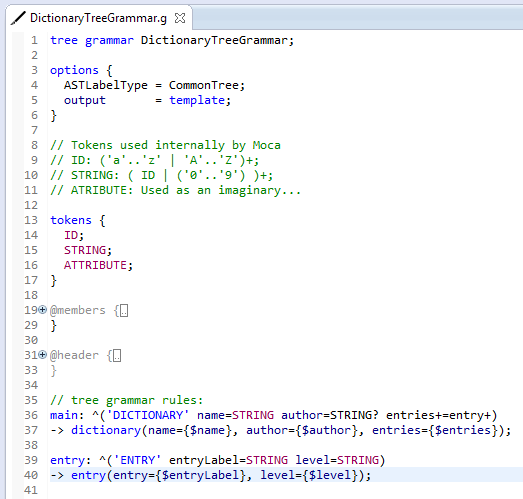
\includegraphics[width=0.8\textwidth]{eclipse_dictionaryTreeGrammar}
  \caption{figureCaption}
  \label{eclipse:treeGrammar}
\end{center}
\end{figure}

\item[$\blacktriangleright$] In the same folder, check out the generated \texttt{DictionaryUnparserAdapter.java} file (FIG). 

This file contains a \texttt{StringTemplateGroup} method for retrieving a group of templates and needs to be implemented. FIG shows the generated comments which
explain how to use either a folder containing different template files, or a single file containing all templates. The latter is better for numerous small
templates, while the former makes sense when the template contains a lot of static text.

\begin{figure}[htpb]
\begin{center}
  %\includegraphics[width=\textwidth]{eclipse_UnparserAdapterNotImplemented}
  \caption{figureCaption}
  \label{eclipse:unparserCommented}
\end{center}
\end{figure}


\item[$\blacktriangleright$] For this our small example, a single file with all templates is ideal. Uncomment line 44 (the option for a group file) and remove
the \texttt{UnsupportedOperationException} command.

\item[$\blacktriangleright$] Now we need to create this template. Navigate to the empty ``templates'' folder of your adapter project and create a new file
called \texttt{Dictionary.stg}. Edit it with the stuff from FIG below.

\begin{figure}[htpb]
\begin{center}
  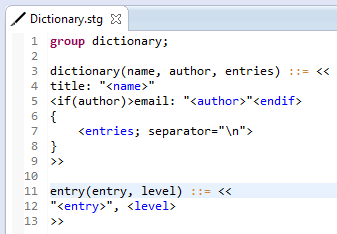
\includegraphics[width=0.5\textwidth]{eclipse_dictionaryTemplate}
  \caption{figureCaption}
  \label{eclipse:dictionaryTemplate}
\end{center}
\end{figure}

\item[$\blacktriangleright$] Our final step is to actually order our TGG to unparse our result, to open \texttt{TGGMain.java}, and uncomment line 46. As you can
see, it will create and place the results of this action into a single ``out'' folder in the instance directory. 

\item[$\blacktriangleright$] Run this file - you should now have the same content in both your input and output files (FIG) Feel free to inspect these files.

\vspace{0.5cm}

\begin{figure}[htpb]
\begin{center}
  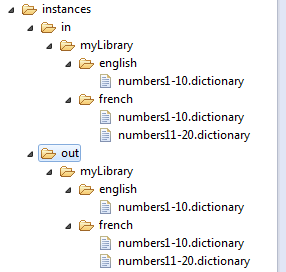
\includegraphics[width=0.5\textwidth]{eclipse_finalInstancesHierarchy}
  \caption{figureCaption}
  \label{eclipse:dictionaryTemplate}
\end{center}
\end{figure}

\item[$\blacktriangleright$] Awesome work - your transformation trip is complete! Play around with changing some of the files such as the unparsing template, or
the content of the ORIGINAL files. How are the results of the transformation affected?

\end{itemize}